\documentclass[tikz,border=4pt]{standalone}
\usepackage{ctex}
\usepackage{amsmath}
\usepackage{pgfplots}
\pgfplotsset{compat=1.18}
\usetikzlibrary{calc, arrows.meta}

\begin{document}
% part14/01 一次函数+反比例函数交点图
% y1 = -x+4, y2 = 3/x; 交于A(1,3)和B(3,1)
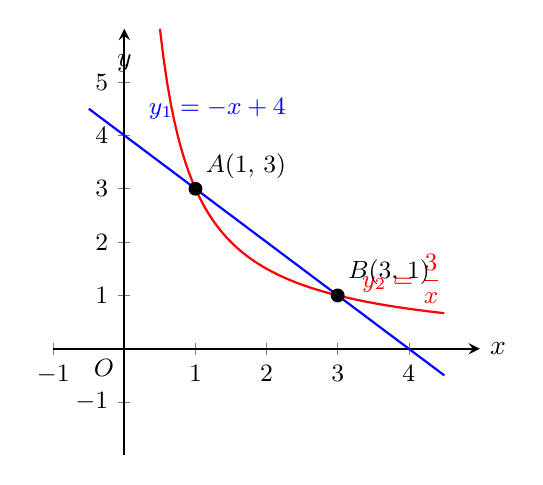
\begin{tikzpicture}
\begin{axis}[
  axis lines=center,
  xlabel={$x$}, ylabel={$y$},
  every axis x label/.style={at={(axis cs:5,0)}, anchor=west},
  every axis y label/.style={at={(axis cs:0,5)}, anchor=south},
  xmin=-1, xmax=5, ymin=-2, ymax=6,
  xtick={-1,0,1,2,3,4},
  ytick={-1,0,1,2,3,4,5},
  tick label style={font=\small},
  width=7cm, height=7cm,
  thick,
]
  % 一次函数 y = -x + 4
  \addplot[blue, thick, domain=-0.5:4.5, samples=50] {-x+4};
  \node[blue, right, font=\small] at (axis cs:0.2,4.5) {$y_1=-x+4$};

  % 反比例函数 y = 3/x（第一象限）
  \addplot[red, thick, domain=0.5:4.5, samples=80] {3/x};
  % 反比例函数（第三象限）
  \addplot[red, thick, domain=-1:-0.5, samples=20] {3/x};
  \node[red, right, font=\small] at (axis cs:3.2,1.3) {$y_2=\dfrac{3}{x}$};

  % 交点A(1,3)
  \fill (axis cs:1,3) circle(2.5pt);
  \node[above right, font=\small] at (axis cs:1,3) {$A(1,\,3)$};

  % 交点B(3,1)
  \fill (axis cs:3,1) circle(2.5pt);
  \node[above right, font=\small] at (axis cs:3,1) {$B(3,\,1)$};

  % 原点
  \node[below left, font=\small] at (axis cs:0,0) {$O$};
\end{axis}
\end{tikzpicture}
\end{document}
